


% \documentclass[a4paper]{article}
\documentclass[12pt,twoside,onecolumn]{article}
\usepackage{a4}
\usepackage{graphicx, fullpage, float, subfig, verbatim,amsmath, multirow, fancyhdr, hyperref}
\usepackage[utf8]{inputenc} 
\usepackage[norsk]{babel}
\usepackage{empheq}
\usepackage[dvipsnames,table]{xcolor}


%\title{\textbf{''Gisse GIS''  \\- webbasert geografisk informasjonssytem ved hjelp av Open Source-programvare}
%\\ \normalsize TBA 4251 - Programmering i geomatikk, høsten 2012}
%\author{Steffen Pøhner Henriksen}
%\date{\today}

\makeatletter
\def\thickhrulefill{\leavevmode \leaders \hrule height 1pt\hfill \kern \z@}
\def\maketitle{%
  \null
  \thispagestyle{empty}%
  \vskip 1cm
  \begin{flushright}
    \normalfont\huge\@title\par
  \end{flushright}
  \vfil
  \begin{flushright}
    \LARGE \strut \@author \par
  \end{flushright}
  \par
  \vfil
  \vfil
  \null
  }
\makeatother
\title{\textbf{''Gisse GIS''  \\- webbasert geografisk informasjonssytem ved hjelp av\\ Open Source-programvare}
\\ \normalsize TBA 4251 - Programmering i geomatikk, høsten 2012}
\author{Steffen Pøhner Henriksen}
\date{\today}
\begin{document}
\maketitle

\vspace{3cm}

\pagebreak

\begin{abstract}

	Gisse GIS er resultatet av min innsats i faget "TBA4251 - Programmering i geomatikk". Det er et enkelt geografisk informasjonssystem som kjører i en nettleser. Ved hjelp av Open Source-programvare vises vektordata over fritt tilgjenglige bakgrunnskart. Vektordataene kan så manipuleres med metoder kjent fra kraftfulle GIS som er desktop-applikasjoner. Metodene som støttes i dag er:
	
	\begin{itemize}
		\item Buffer - Utvider valgt område med en gitt verdi i meter.
		\item Area - Gir arealet av området i kvadratmeter.
		\item Merge - Slår sammen to vektorlag.
		\item Subtract - Trekker et vektorlag fra et annet.
		\item Intersect - Returnerer overlappende vektorlag.
		\item Distance - Finner minste avstand mellom to vektorlag.
		\item Simplify - Forenkler geometrien til et vektorlag ved Douglas-Peuker. 
	\end{itemize}
	
	Programmet består av tre deler - database, serverlag og klient. Kommunikasjonen mellom server og klient skjer via Websockets\cite{websockets}. Klienten er skrevet i Javascript, med HTML5 og CSS3. Tilleggsbiblioteker som er brukt i klienten er Knockout.js og jQuery, samt Twitter Bootstrap. Serverlaget er skrevet i node.js som tilbyr Javascript til bruk for serverkode. Her er sockets.io, Express og databasedriver brukt som tilleggsbiblioteker. Eksempeldata brukt i utviklingen og til demostrasjon er hentet fra Open Street Map og lagres i en PostgreSQL-database med PostGIS-utvidelse. Alt er lagret i skyen hos Amazons EC2-tjeneste, som sørger for at programmet leveres til brukers nettleser. 
	
	Resultatet er et brukervennlig GIS som utfører enkle operasjoner vi kjenner fra før, på frie vektordata som eksempel. ''Gisse GIS'' kan prøves ved å besøke adressen http://gisse.pohnerhenriksen.com i din nettleser.
	
\end{abstract}
\newpage

\tableofcontents
\newpage

\section{Innledning}
	
	Denne rapporten omhandler arbeidet med ''Gisse GIS'' utført høsten 2012. Den er et resultat av faget ''TBA4251 - Programmering i Geomatikk'' ved NTNU. Rapporten argumenterer for valg av programmeringsspråk, tilleggsbiblioteker og fremgangsmåte i arbeidsprosessen. Dataflyt og strukturen av programmet blir lagt frem. Et forslag til et scenario for å teste programmet blir også presentert. Oppdagede bugs, feil og mangler blir listet opp og kommentert. 
	
	Man kan dele inn arbeidet i fire deler - design, implementering, bugfiksing og rapportskriving. En stor del av arbeidet med utarbeidelsen av programmet var definere hva det skulle bli, hvilke verktøy som var hensiktsmessig å bruke, samt lære seg disse verktøyene. Tidlig ble det bestemt at jeg ville velge GIS-oppgaven i faget. Det gav meg muligheten til å jobbe med Javascript/HTML, noe jeg ikke har brukt i noen særlig grad før og har lyst til å lære meg. Oppgaven er farget av at jeg i størst mulig grad ville benytte meg av Open Source-programvare, og gjøre meg kjent med hva som finnes av slik programvare for bruk i geomatikkfaget. 
	
	\begin{quotation}
		"Software is like sex: it's better when it's free." 
			\em  -- Linus Torvalds
	\end{quotation}
	
	Tidligere har jeg jobbet hos Norkart AS som systemutvikler. Her laget jeg en database/server-løsning som behandlet geografiske data med tilleggsinformasjon. Kunnskapen fra denne sommerjobben kom godt med i utarbeidelsen av oppgaven. Kunnskapen opparbeidet herfra gjorde at jeg raskt så muligheter som PostGIS gir, og at implementeringen av databasedelen gikk relativt lett.
	
	\begin{figure}[h]
	\centering
	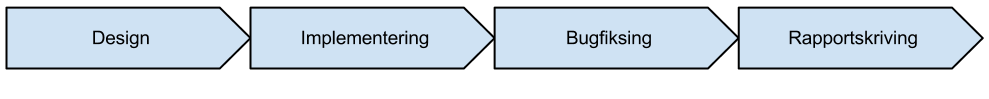
\includegraphics[scale=0.5]{innledning.png}
	\caption[Arbeidsprosess]{Arbeidsprosess}
	\end{figure}
	
\section{Formål med applikasjonen}

	Applikasjonen tilbyr brukeren et GIS med grunnleggende funksjoner som er tilgjenglig uavhengig av plattform. Den kjøres i alle moderne nettlesere. Det gjør ''Gisse GIS'' lett tilgjenglig, og enkelt å ta i bruk da det ikke krever noen installasjon utover å besøke en nettadresse. Funksjonene utføres raskt, og krever lite av klienten. Det er serveren som står for kalkulasjonene. Applikasjonen er ment som en inngansportal, og et demonstrasjonsverktøy for GIS. Man kan enkelt ved hjelp av åpne eksempeldata vise hvor kraftfullt et geografisk informasjonssytem kan være ved hjelp av enkle funksjoner. 
	
	Undertegnede håper også at kodegrunnlaget kan være et springbrett for andre studenter og GIS-interesserte til å lage nettbaserte kartløsninger. Kildekoden ligger fritt tilgjenglig på Github, og kan brukes fritt under OpenSource-lisensen. 
	
	I tillegg til funksjonene man kan utføre på vektordata er også mange ulike bakgrunnskart vist frem i applikasjonen. Disse kan brukes uavhengig av resten av programmet. Både kart, hybridkart og satelittbilder er tilgjenglig. Det finnes få eksempler på implementasjon av Kartverkets kart i websammenheng, og jeg håper koden kan hjelpe flere i å ta i bruk disse. Bedre kart finnes jo ikke over Norge! Og altfor få norske kartapplikasjoner tar i bruk Kartverkets kart. 

\section{Valg av programmeringsspråk}
	
	Jeg var aldri i tvil om at det var GIS-oppgaven jeg ville velge. For å kunne nå ut til flest mulig brukere, uavhengig av maskinvarekonfigurasjon og plattform ville jeg bruke nettleseren. Da kunne også applikasjonen fungere på smarttelefoner og nettbrett i tillegg til desktop. Og dette uten å lage egne apps for disse.
	
	\subsection{HTML5 og CSS3}
		
		Med nettleseren som klient kommer man ikke unna HTML og CSS for å henholdsvis strukturere og designe en nettside. Jeg valgte å ta i bruk den nyeste standarden av HTML, HTML5. Dette gjorde det mulig å ta i bruk canvas-elementet for å tegne kart, og bruke rask nettverksoverføring via Websockets. Dette gjør at opplevelsen for brukeren med en moderne nettleser blir best mulig. HTML5 er også standarden i dag, og jeg fant det best å lære seg denne versjonen.
		
		CSS3 tilbyr en del nye funksjoner i forhold til den eldre CSS 2.0. Jeg har ikke tatt i bruk altfor mange av disse nye funksjonene, men gjort meg litt kjent med mulighetene. I applikasjonen har jeg rundet av hjørnene på menyene med kommandoer hentet fra CSS3. Dette skaper et mer helhetlig, rent og funksjonelt design. 
	
		\subsubsection{Twitter Bootstrap}
			
			Grunnet prosjektets tidsbegrensning og for enkelhetens skyld brukte jeg et rammeverk for å sette opp hjemmesiden. Dette heter Twitter Bootstrap, og gir muligheten til å bruke en hel del forhåndsdesignede elementer. Rammeverket er svært populært. Med dette kunne jeg lage navigeringsstripa på toppen, samt design på knapper. Hjelpesiden, og ''om meg'' involverer sterk bruk av dette rammeverket. Verktøymenyene er derimot laget spesielt for denne siden. Rammeverket er svært nyttig for såkalt "responsivt design". På den måten kan man lage nettsider som ser bra ut på store og små skjermer, også smarttelefoner og nettbrett. 
			
		\subsubsection{Leaflet}
		
			Kartet på siden tegnes av javascriptbiblioteket Leaflet. Dette er et nytt og moderne alternativ til det mer kjente Open Layers. Leaflet er kjent for å være bedre på små skjermer, samt enklere å bruke. Den tar i bruk canvas-elementet i HTML5. Jeg bruker Leaflet til å tegne GeoJSON-filer fra som mottas fra serveren, vise bakgrunnskart og popup-elementer. Den fungerer fint på nettbrett og smarttelefoner da klype-zoom støttes. Bakgrunnskart som er tilgjenglig er:
			
			\begin{itemize}
				\item Karverkets topografiske kart (farge og sort/hvitt)
				\item Karverkets topografiske rasterkart
				\item Cloudmade
				\item MapQuest
				\item OpenStreetMap
				\item Google (roadmap, satelitt og hybrid)
				\item To kreative kart
				\item Bing-satelittbilder
				\item MapQuest satelittbilder
			\end{itemize}
			
	\subsection{JavaScript}
	
		JavaScript brukes for å gi dynamisk innhold til nettsider, og er et naturlig valg i enhver webapplikasjon. Dette er et språk som bare blir mer og mer populært, og er spådd en stor fremtid. ''Gisse GIS'' tar i bruk javascript i mange deler av programmet. Og står for selve kjernen av koden. 
		
		\subsubsection{jQuery}
		
		jQuery er et støttebibliotek til javascript. Det finnes knapt javascript som ikke tar i bruk dette. Det forenkler kodeflyten, og kommandoene i javascript. Biblioteket legger flere og enklere verktøy i verktøykasse til webutvikleren. jQuery blandt annet for animasjonene av menyene, pekere på dynamisk innhold og menyhåndtering.
		
		\subsubsection{Knockout.js}
		
		Knockout.js implementerer Model-View-View-Model (MVVC) på en enkel måte i applikasjonen. Den holder styr på vektorlagene, og oppdaterer brukergrensesnittet om den oppdager noen endringer. 
		
		\subsubsection{Node.js}
		\subsubsection{socket.io}
	\subsection{PostgreSQL - PostGIS}

\section{Server i skyen - Amazon EC2}

\section{Testscenario}
\section{Bugs, feil og mangler}
	\subsection{Forbedringspotensiale}
\section{Diskusjon - Løser applikasjonen oppgaven?}

\newpage
\begin{thebibliography}{9}

\bibitem{websockets}
	Wikipedia: Websockets, http://en.wikipedia.org/wiki/WebSocket, 22.12.2012

\end{thebibliography}

\listoffigures

\end{document}

